\definecolor{darkgreen}{rgb}{0,.6,0}
  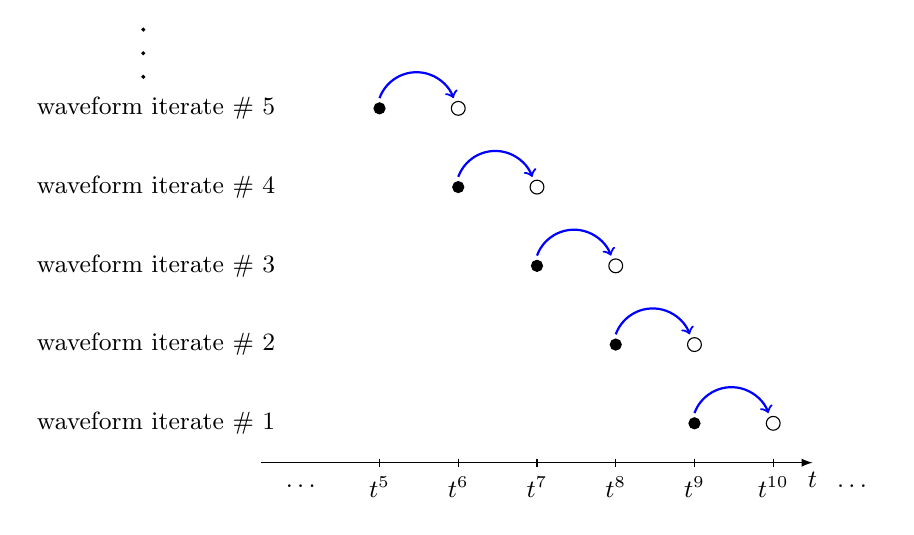
\begin{tikzpicture}[scale=1.0]
    % background grid
    %\draw[step=.2,gray,very thin] (-2.3,-.35) grid (4.4,3.4);

    % \tikzstyle{my style}=[draw=#1,fill=#1!20]
    \tikzstyle{dropline_style}=[densely dotted,thin]

%    \draw[shift={(0.5,2)},dropline_style]  (0,-0.2) -- ++(0,-0.8);
%    \draw[shift={(1.2,2)},dropline_style]  (0,-0.2) -- ++(0,-0.8);

%    \draw[shift={(0.5,3)},dropline_style]  (0,-0.2) -- ++(0,-0.8);
%    \draw[shift={(0,3)},dropline_style] (0,-0.2) -- ++(0,-0.8);

%    \draw[shift={(2.5,1)},dropline_style]  (0,-0.2) -- ++(0,-0.8);
%    \draw[shift={(1.2,1)},dropline_style]  (0,-0.2) -- ++(0,-0.8);


    %\foreach \x/\xtext in {-1, -0.5/-\frac{1}{2}, 1}
    %\draw (\x cm,1pt) -- (\x cm,-1pt) node[anchor=north] {$\xtext$};

    \draw (-2.2, 0) node[left] {\small waveform iterate \# 1};
    \draw (-2.2, 1) node[left] {\small waveform iterate \# 2};
    \draw (-2.2, 2) node[left] {\small waveform iterate \# 3};
    \draw (-2.2, 3) node[left] {\small waveform iterate \# 4};
    \draw (-2.2, 4) node[left] {\small waveform iterate \# 5};


    % position of the time-line
    \def\y{-0.5}
    \draw [-latex] (-2.5,\y) -- (4.5,\y);

    \def\tick{0.05}
    \draw (4.5,\y) node[below] {\small $t$};
    \draw (-2,\y) node[below] {\small \phantom{t}$\ldots$\phantom{t}};
    \draw (-1,\y) ++(0,\tick) -- ++(0,-2*\tick) node[below] {\small $t^{5}$};
    \draw (0,\y) ++(0,\tick) -- ++(0,-2*\tick) node[below] {\small $t^{6}$};
    \draw (1,\y) ++(0,\tick) -- ++(0,-2*\tick) node[below] {\small $t^{7}$};
    \draw (2,\y) ++(0,\tick) -- ++(0,-2*\tick) node[below] {\small $t^{8}$};
    \draw (3,\y) ++(0,\tick) -- ++(0,-2*\tick) node[below] {\small $t^{9}$};
    \draw (4,\y) ++(0,\tick) -- ++(0,-2*\tick) node[below] {\small $t^{10}$};
    \draw (5,\y)  node[below] {\small \phantom{t}$\ldots$\phantom{t}};


    % parameters for stencil diagrams
    \def\rad{0.12}
    \def\omr{0.88}   % 1-rad
    \def\intthick{0.068}   % thickness of integral bars

    % filled dots
    \foreach \xy in { (3,0),(2,1),(1,2),(0,3),(-1,4) }
    \filldraw \xy circle (2pt);

    % hollow dots
    \foreach \xy in { (4,0),(3,1),(2,2),(1,3),(0,4) }
    \filldraw[fill=white] \xy circle (2.5pt);

    % arrows
    \draw [->,thick,blue] (-1,4.13) arc (160:20:0.5 and 0.5);
    \draw [->,thick,blue] (0,3.13) arc (160:20:0.5 and 0.5);
    \draw [->,thick,blue] (1,2.13) arc (160:20:0.5 and 0.5);
    \draw [->,thick,blue] (2,1.13) arc (160:20:0.5 and 0.5);
    \draw [->,thick,blue] (3,0.13) arc (160:20:0.5 and 0.5);

    % dots for more waveform iterates
    \foreach \xy in { (-4,4.4),(-4,4.7),(-4,5.0) }
    \filldraw \xy circle (0.5pt);

  \end{tikzpicture}
